%% LyX 2.2.1 created this file.  For more info, see http://www.lyx.org/.
%% Do not edit unless you really know what you are doing.
\documentclass[12pt,english,ngerman,british,pointlessnumbers, abstracton, headsepline]{scrreprt}
\renewcommand{\familydefault}{\sfdefault}
\usepackage[T1]{fontenc}
\usepackage[latin9]{inputenc}
\usepackage{geometry}
\geometry{verbose,tmargin=2.5cm,bmargin=2.5cm}
\pagestyle{plain}
\setlength{\parskip}{\medskipamount}
\setlength{\parindent}{0pt}
\usepackage{array}
\usepackage{verbatim}
\usepackage{float}
\usepackage{multirow}
\usepackage{amsmath}
\usepackage{amsthm}
\usepackage{graphicx}
\usepackage{setspace}
\setstretch{1.2}

\makeatletter

%%%%%%%%%%%%%%%%%%%%%%%%%%%%%% LyX specific LaTeX commands.
%% Because html converters don't know tabularnewline
\providecommand{\tabularnewline}{\\}
\floatstyle{ruled}
\newfloat{algorithm}{tbp}{loa}[chapter]
\providecommand{\algorithmname}{Algorithm}
\floatname{algorithm}{\protect\algorithmname}

%%%%%%%%%%%%%%%%%%%%%%%%%%%%%% User specified LaTeX commands.
% verschieden Symbole, Zeichen wie (c), �
\usepackage{textcomp,units}

% Mehr Platz zwischen Tabelle und Untertitel
\usepackage{caption}
\usepackage{subcaption}
\captionsetup[table]{skip=10pt}

%Kapitelzahl sehr gro�
\makeatletter% siehe De-TeX-FAQ 
 \renewcommand*{\chapterformat}{% 
   \begingroup% damit \unitlength-�nderung lokal bleibt 
     \setlength{\unitlength}{1mm}% 
     \begin{picture}(10,10)(0,5) 
       \setlength{\fboxsep}{0pt} 
       %\put(0,0){\framebox(20,40){}}% 
       %\put(0,20){\makebox(20,20){\rule{20\unitlength}{20\unitlength}}}% 
       \put(10,15){\line(1,0){\dimexpr 
           \textwidth-20\unitlength\relax\@gobble}}% 
       \put(0,0){\makebox(10,20)[r]{% 
           \fontsize{28\unitlength}{28\unitlength}\selectfont\thechapter 
           \kern-.05em% Ziffer in der Zeichenzelle nach rechts schieben 
         }}% 
       \put(10,15){\makebox(\dimexpr 
           \textwidth-20\unitlength\relax\@gobble,\ht\strutbox\@gobble)[l]{% 
             \ \normalsize\color{black}\chapapp~\thechapter\autodot 
           }}% 
     \end{picture} % <-- Leerzeichen ist hier beabsichtigt! 
   \endgroup 
}

\usepackage{ %a4wide,
            ellipsis, fixltx2e, mparhack,   %Fehlerkorrektur f�r Marginalien
            booktabs, longtable             %sch�nere Tabellen
}  

\usepackage[automark]{scrpage2}
%\automark[chapter]{chapter}
\clearscrheadfoot
\ohead{\\\headmark}
\ihead{\includegraphics[scale=0.15]{logo.jpg}}%\pagemark}
\ofoot[\pagemark]{\pagemark}


%Kurzfassung und Abstract (englisch) auf eine Seite
\renewenvironment{abstract}{
    \@beginparpenalty\@lowpenalty
      \begin{center}
        \normalfont\sectfont\nobreak\abstractname
        \@endparpenalty\@M
      \end{center}
}{
    \par
}



% sch�nerer Blocksatz!!
\usepackage{microtype}

\usepackage{ifpdf} % part of the hyperref bundle
\ifpdf % if pdflatex is used

%set fonts for nicer pdf view
 \IfFileExists{lmodern.sty}{\usepackage{lmodern}}
  {\usepackage[scaled=0.92]{helvet}
    \usepackage{mathptmx}
    \usepackage{courier} }
\fi

 % the pages of the TOC are numbered roman
 % and a pdf-bookmark for the TOC is added
 \pagenumbering{arabic}
 \let\myTOC\tableofcontents
 \renewcommand\tableofcontents{
   %\pdfbookmark[1]{Contents}{}
   \myTOC
   \clearpage
   \pagenumbering{arabic}}

%Bezeichungen anpassen
%Babelpaket mu� zuvor geladen werden
%\usepackage[ngerman]{babel}
%\addto\captionsngerman{ 
%\renewcommand{\figurename}{Abb.}% 
%\renewcommand{\tablename}{Tab.}% 
%\renewcommand{\abstractname}{Kurzfassung}
%\renewcommand{\nomname}{Abk�rzungen}
%}

% Alle Querverweise und URLs als Link darstellen
% In der PDF-Ausgabe
 \usepackage[colorlinks=true, bookmarks, bookmarksnumbered, bookmarksopen, bookmarksopenlevel=1,
  linkcolor=black, citecolor=black, urlcolor=blue, filecolor=blue,
  pdfpagelayout=OneColumn, pdfnewwindow=true,
  pdfstartview=XYZ, plainpages=false, pdfpagelabels,
  pdfauthor={LyX Team}, pdftex,
  pdftitle={LyX's Figure, Table, Floats, Notes, and Boxes manual},
  pdfsubject={LyX-documentation about figures, tables, floats, notes, and boxes},
  pdfkeywords={LyX, Tables, Figures, Floats, Boxes, Notes}]{hyperref}
% algorithm package
\usepackage{algorithm,algpseudocode}

%mehr Platz zwischen �berschrift und Tabelle
\newcommand{\@ldtable}{}
\let\@ldtable\table
\renewcommand{\table}{ %
                 \setlength{\@tempdima}{\abovecaptionskip} %
                 \setlength{\abovecaptionskip}{\belowcaptionskip} %
                 \setlength{\belowcaptionskip}{\@tempdima} %
                 \@ldtable}
% for better tables
\usepackage{caption, booktabs}

\renewcommand\[{\begin{equation}}
\renewcommand\]{\end{equation}}

\usepackage{color, colortbl}
\definecolor{LightCyan}{rgb}{0.88,1,1}

\usepackage{url}
%In dieser Arbeit wird auf die Nomenklatur als Abk�rzungsverzeichnis verzichtet. Bei Wunsch wieder aktivieren.
%Nomenklatur als Abk�rzungsverzeichnis verwenden
%\renewcommand{\nomname}{Abk�rzungsverzeichnis}
%\renewcommand{\nomlabelwidth}{20mm}

%Nomenklatur als Glossar verwenden
%Nur Noetig wenn auch Glossar verwendet wird.
%\renewcommand{\nomname}{Glossar}

%Farbe f�r Programmcode festlegen
 

\AtBeginDocument{
  \def\labelitemiii{\(\circ\)}
}

\makeatother

\usepackage{babel}
\addto\captionsenglish{\renewcommand{\algorithmname}{Algorithm}}
\addto\captionsngerman{\renewcommand{\algorithmname}{Algorithmus}}

\begin{document}
\titlepage

\begin{center}
\begin{tabular}{lc}
 & \multirow{5}{*}{\includegraphics[width=7.5cm]{images/UniOsnabr�ck}}\tabularnewline
Fakult�t Humanwissenschaften\hspace{2.5cm} & \tabularnewline
 & \tabularnewline
 & \tabularnewline
 & \tabularnewline
\end{tabular}
\par\end{center}

\vspace{7cm}

\begin{flushleft}
\textbf{\Large{}Bachelor thesis}
\par\end{flushleft}{\Large \par}

\begin{flushleft}
{\large{}Adaptive K-Means Clustering of Data Sequences}
\par\end{flushleft}{\large \par}

Clustering of video sequences with dynamic cluster count and recognition
of their serial identity

\begin{flushleft}
{\Large{}\vspace{1.5cm}
}
\par\end{flushleft}{\Large \par}

\begin{tabular}{ll}
eingereicht von:\hspace{1cm} & Linus Edelkott \tabularnewline
 & Matrikelnummer: 950499\tabularnewline
 & Studiengang: Cognitive Science\tabularnewline
 & Universit�t Osnabr�ck\tabularnewline
 & \tabularnewline
Betreuer: & MS Julius Sch�ning\tabularnewline
 & Universit�t Osnabr�ck\tabularnewline
 & Prof. Dr. Gunther Heidemann\tabularnewline
 & Universit�t Osnabr�ck\tabularnewline
 & \tabularnewline
\multicolumn{2}{l}{Osnabr�ck, \today}\tabularnewline
\end{tabular}

\begin{flushleft}
\newpage{}
\par\end{flushleft}

\selectlanguage{ngerman}%
~

\vspace{17.1mm}

\begin{flushleft}
\textbf{\huge{}Declaration of authorship}
\par\end{flushleft}{\huge \par}

I hereby certify that the work presented here is, to the best of my
knowledge and belief, original and the result of my own investigations,
except as acknowledged, and has not been submitted, either in part
or whole, for a degree at this or any other university.

\vspace{2cm}

\begin{center}
\begin{tabular*}{15cm}{@{\extracolsep{\fill}}cl}
Osnabr�ck, \today & \selectlanguage{british}%
\begin{comment}
Unterschrift
\end{comment}
\selectlanguage{ngerman}%
\tabularnewline
\selectlanguage{british}%
\selectlanguage{ngerman}%
 & \selectlanguage{british}%
Linus Edelkott\selectlanguage{ngerman}%
\tabularnewline
\end{tabular*}
\par\end{center}

\newpage{}

\selectlanguage{british}%
\tableofcontents{}

\newpage{}

\listof{algorithm}{List of Algorithms}

\newpage{}

\listoffigures

\newpage{}

\pagenumbering{arabic}
\setcounter{page}{3}

\renewcommand{\chaptername}{}

\chapter{Introduction}

K-means clustering is one of the most often used clustering algorithms
for image segmentation. Image segmentation is the basis for many image
analysis techniques and thus highly values reliable results and computing
time. While k-means clustering offers a great deal for the latter
part, reliable results are sensitive towards the starting positions.
The starting position is defined as the chosen initial cluster number
and their respective position. 

So far there exists no generally acknowledged optimal solution to
compute the optimal number of clusters for any given data set a priori.
One common bypass is to run the algorithm several times with different
starting points. Especially for image segmentation however, many proposals
have been made to create good starting points for clustering images\cite{ChrisSolomon2011_km}.

The goal of this thesis is to adapt one of these algorithms to video
sequences and improve it through the gained knowledge from continuous
frames. The created clusters for each frame should then be compared
to its predecessor, to determine whether clusters of previous frames
persisted. Creating an algorithm to identify good starting positions
for k-means clustering in video sequences can already be used for
video compression on its own, but it could also be useful for many
fields of video analysis as for example feature extraction and object
recognition. If a cluster contains most visible features of an object,
the identification of the serial identity of this particular clusters
can especially be applicable in fields as object tracking.

The organization of this thesis is as follows. Chapter 2 provides
some information on clustering and image segmentation fundamentals.
It introduces k-means clustering and an algorithm to find good starting
positions for k-means clustering in image segmentation.

Chapter 3 specifies the underlying task of this bachelor thesis and
presents the developed procedures and algorithms.

In chapter 4 the results of the performance evaluation are presented
successively on synthetic and real data. Thereby some necessary tweaks
of the proposed algorithm are introduced and implemented.

Chapter 5 reviews the evaluation and concludes the thesis.

\chapter{Theoretical basis}

\section{Clustering}

Clustering can broadly be described as classification of data into
several groups. Clustering algorithms are unsupervised learning algorithms,
which means they make no prior assumptions about the ouput components\cite{Lucchese_colorimage}.

The vague objective is to find ``\textit{interesting} groupings
of training samples``\cite{VladimirCherkassky2007}. This separation
into a number of groups, called clusters, happens according to a measure
of similarity. The goal of the algorithm is to find clusters in a
way, that samples within are more similar to each other than samples
from different clusters and thus minimizing the prediction error.
This is often summarized as the weighting of ``intra-cluster'' and
``inter-cluster'' distance. The first one describes the distinction
from samples within a cluster, whereas the latter is the distance
of one cluster to another one\cite{Ray1999}.

Hereby the similarity measurement reflects a priori knowledge, for
example using standard Euclidean distance on a RGB color space equals
the assumption that all values have equal importance. Nevertheless
is the clustering process usually ,,ad hoc``; the underlying clustering
process defines the relevant information itself. This makes clustering
very generalizable\cite{VladimirCherkassky2007}.

Often clustering algorithms create prototypes. A prototype is a data
object that is representative of all other objects in the cluster.
In most cases this is simply the average of each data point within
the cluster. Protoypes can be used in many ways, they ease the comparison
of clusters among each other and can be used for data compression.
Therefore they are often used as input for further data processing
or data analysis techniques\cite{Pang-NingTan2005}.

One of the most common usage of clustering algorithms is dimensionality
reduction. The goal is to find a mapping from a $d-$dimensional input
space $R^{d}$to some $m$ dimensional output space $R^{m}$, where
$m<d$\cite{VladimirCherkassky2007}.

\[
G(x):R^{d}\rightarrow R^{m}
\]

A good mapping should also possess the inverse function.

\[
F(z)=R^{m}\rightarrow R^{d}
\]

Hence the reduced output can be decoded to the original input without
losing to much information. Thus the main features can be kept, while
the amount of data is reduced.

Clusters can either be described hierarchically (i.e. described in
tree structures) or they can be purely partitional. The latter sort
can be further divided into 2 groups. The first one is called ,,hard
clustering``, each sample is definitely placed in only one cluster.
The second one is called ,,soft clustering`` and in alternative
each sample can belong to serveral clusters according to a related
probability distribution.\cite{Poole2010}

\section{K-means clustering}

K-means clustering is one of the oldest and most widely used clustering
algorithms. It requires an explicit distance measure, an input of
training samples and the number of classes k. It belongs to the class
of hard clustering algorithms.\cite{Poole2010} 

The main concept is to represent each cluster by the vector of mean
attribute values for numeric attributes or by a vector of the most
frequent values for nominal attributes that are assigned to that cluster\cite{IBM_BigInsights}.
In contrast to numeric values, nominal attributes can not simply be
ordered and have only a limited set of values. This kind of representation
is also called cluster center and acts as a prototype.\cite{Pang-NingTan2005}

The operation of k-means clustering can be seen in algorithm 2.1.
It starts with initializing random points as centroid of a cluster.
This initialization process will be repeated until the desired number
K of clusters is generated. The next step is to assign every training
sample to the closest cluster center and update it by shifting it
to the mean of all cluster members for each attribute. This step has
to be repeated until it converges, due to bad initialization points
this might take many iterations. Hence the usual implementation either
uses a limit for the number of iterations or stops if the number of
changes fall below a certain $\epsilon$. 

\begin{algorithm}[H]
\caption{Basic K-means algorithm}

\begin{algorithmic}[1]
\State {select K points as initial centroids}
\Repeat {}
\State {assign each data sample to the closest center}
\State {update the cluster centers by shifting them to the mean of each attribute}
\Until {centroids moved no more than $\epsilon$}
\end{algorithmic}
\end{algorithm}

\begin{figure}[H]
\begin{subfigure}[c]{0.5\textwidth} 
\frame{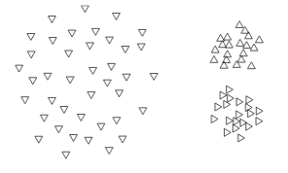
\includegraphics[width=\textwidth]
{/home/nilus/Dokumente/LyxBachelorarbeit/Bachelorarbeit/images/example_kmeans.png}}
\subcaption{Original points} 
\end{subfigure}
\begin{subfigure}[c]{0.5\textwidth} 
\frame{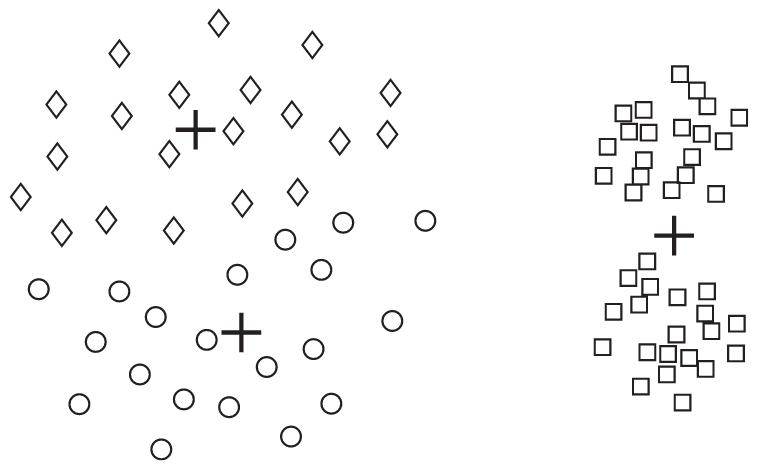
\includegraphics[width=1\textwidth]
{/home/nilus/Dokumente/LyxBachelorarbeit/Bachelorarbeit/images/example_kmeans_original.png}}
\subcaption{Cluster centers with k = 3} 
\end{subfigure}

\caption{Example of k-means clustering on data with distinct groups\cite{Pang-NingTan2005}}
\end{figure}

The k-means algorithm aims to minimize an objective squared error
function: 

\[
J=\sum_{j=1}^{k}\sum_{\forall i}|x_{i}^{j}-c_{j}|^{2}
\]
hereby $c_{j}$ is the coordinate vector of the $j$th cluster, $\{x_{i}^{j}\}$
are the points assigned to the $j$th cluster and $|x_{i}^{j}-c_{j}|$
describes the distance\cite{ChrisSolomon2011_km}. It can be shown
that the k-means algorithm converges to a local minimum\cite{Fu1981}.

The relevant distance measure can be chosen dependent on the task,
but most of the times the normal Euclidean distance is used. \\
\[
\text{Euclidean distance: }\frac{1}{I}\cdot\forall i\left(\sqrt{x_{i}-c_{i}}\right)^{2}
\]

An advange of k-means clustering is its low complexity but it has
some weaknesses. K-means struggle with outliers, which highly influence
the results. It can also only be used on data for which there is a
centroid and it cannot handle non-globular clusters as seen in Figure
2.2. Finally it has the requirement of getting an accurate number
of clusters as input a priori\cite{Bora2015,Pang-NingTan2005}.

\begin{figure}[H]
\begin{subfigure}[c]{0.5\textwidth} 
\frame {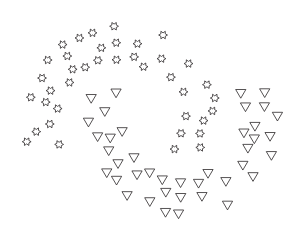
\includegraphics[width=\textwidth]
{/home/nilus/Dokumente/LyxBachelorarbeit/Bachelorarbeit/images/example_kmeans_noglobal_source.png}}
\subcaption{Original points} 
\end{subfigure}
\begin{subfigure}[c]{0.5\textwidth} 
\frame {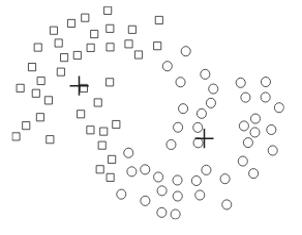
\includegraphics[width=1\textwidth]
{/home/nilus/Dokumente/LyxBachelorarbeit/Bachelorarbeit/images/example_kmeans_noglobal.png}}
\subcaption{Cluster centers with k = 3} 
\end{subfigure}\caption{Example of k-means clustering on data with non-globular clusters\cite{Pang-NingTan2005}}
\end{figure}


\section{Image color segmentation}

One of the many applications for the k-means clustering algorithm
is color segmentation. Image segmentation in general is the process
of splitting/classifying an image into several parts, so that each
region builds a homogenous segment. Combining any of the homogenous
segments would result in a heterogenous segment\cite{Bora2015} .

Segmentation algorithms are often the very first step in image processing.
Subsequent steps as for example feature extraction and classification
are highly reliant on the successful generation of homogenous parts.
If the respective object can not be identified, it can certainly not
be classified. The segmentation outcome will always be dependent on
the underlying image and the object, or feature which should be identified.
Therefore there is no single perfect clustering for an image, this
complicates the evaluation process\cite{ChrisSolomon2011}.

Segmentation algorithm can be divided into two main groups. The first
one is the edge/boundary group; the associated algorithms aim to detect
edges to find boundaries in between groups of pixels. The second group
is region based and tries to order pixels according to their mutual
similarity\cite{ChrisSolomon2011} .

Color image segmentation is usually residing in the second group.
Combined with texture segmentation, it is mostly used in tasks concerned
about content based retrieval\cite{Lucchese_colorimage}. Hereby images
are organised/searched according to their pictured content. 

Clustering algorithms share the same problem as region based segmentation
and can thus be used for color segmentation. The problem of using
k-means clustering for image segmentation is once again the requirement
to assing the number of clusters beforehand. If a good number of clusters
is known however it is optimal in minimizing the average distortion\cite{Park1998}.

\section{Finding the optimal numbers of clusters for k-means clustering}

Although the k-means clustering is relatively easy to implement on
a relative wide field, it has some drawbacks. The final results of
the clustering algorithm vary depending on the number of clusters
and especially on their initialization. So if the initial clusters
are chosen randomly, it will lead to different results\cite{IMCIP-2015}.

In order to find the optimal number of clusters and initialize them
automatically Siddheswar Ray and Rose H. Turi proposed an algorithm
which uses ``a simple validity measure based on the intra-cluster
and inter-cluster distance measure''\cite{Ray1999}. 

The basic k-means algorithm minimizes the sum of squared distanced
from all points to their cluster centers, hence the distances from
each point to their cluster centers provides the information whether
the clusters are compact. The averages of all these distances constitute
the intra-cluster measurement.

\[
\text{intra}=\frac{1}{N}\sum_{i=1}^{K}\|x-z_{i}\|^{2}
\]

where $N$ is the number of all pixels, $K$ is the cluster count
and $z_{i}$ is the actual cluster center. To be as compact as possible,
we obviously want to minimize this measurement. The inter-cluster
measurement in contrast describes the distances between the cluster
centers and should be maximized. 

\[
\text{inter}=\min\left(\|z_{i}-z_{j}\|^{2}\right),i=1,2,...,K-1,j=i+1,...,K
\]

Only the minimum of each distance is considered, because we always
want to maximize the smallest distances. The maximized values of larger
values will be automatically larger as well.

In an optimal clustering we obviously want to have compact clusters,
which are as distant as possible. Thus the validity measurement is
defined as the ratio of the intra and inter measure.

\[
\text{validity}=\frac{\text{intra}}{\text{inter}}
\]

The optimal cluster count should posses the smallest validity. 

The proposed algorithm of Siddheswar Ray and Rose H. Turi can be seen
in algorithm 2.2. It starts with initialising every single data point
into one cluster and using the average of each data point as cluster
center (line 1). Repeatedly the variance of each data point will be
calculated and added up, the sum of all points will be used as divisor
(line 3). The cluster with the largest value will be split (line 4).
Due to the occurring minimization of intra-cluster distance in k-means
clustering, this cluster would most likely be split when increasing
the cluster count. Before the process will be repeated, the normal
k-means clustering is executed and the validity calculated according
to the new calculated cluster centers (line 5). This processes is
repeated until a self-assigned number of clusters $k_{\text{max}}$
is reached. From this follows that the basic k-means algorithm will
be run $k_{\text{max}}$ times.

The clusters will be split, according to the old cluster center and
with regard to the minimum and maximum of each attribute.

\[
z_{i}^{'}=\left(z_{i1}-a_{1},z_{i2}-a_{2},z_{i3}-a_{3}\right)
\]

\[
z_{i}^{''}=\left(z_{i1}+a_{1},z_{i2}+a_{2},z_{i3}+a_{3}\right)
\]

With $z_{i}^{'}$ and $z_{i}^{''}$ being the two new cluster centers,
$z_{i}$ being the the old cluster centers with index $1,2,3$ for
each attribute. 

\[
a_{j}=\frac{z_{ij}-\max_{j}}{2}
\]

Where $\max_{j}$ is the maximum value for the $j$-component.

\begin{algorithm}[H]
\caption{Find the optimal cluster count algorithm}

\begin{algorithmic}[1]
\State {Initialise a single cluster, with the average of each attribute as cluster center}
\Repeat{}
\State {calculate the variance of each attribute $\sigma_{i}$ and add them up $\sum_{i=1}^{I}\frac{1}{I}\sigma_{i}$ }
\State {split the cluster centers with the biggest variance}
\State {use the standard k-means algorithm and calculate the validity}
\Until {a self-assinged limit $k_\text{max}$ is reached}
\end{algorithmic}
\end{algorithm}

Due to the larger inter-cluster distance, small cluster numbers tend
to be selected more often. In synthetic images, with an actual perfect
cluster count the calculated minimal validity will be the optimal
cluster count. In natural images the best number of clusters is usually
prefered. To overcome the effect of a large inter-cluster distance
with a small k, the first local maximum in the validity measure needs
to be found. 

\[
\text{val}(k-1)<\text{val}(k)>\text{val}(k+1)
\]

The adjusted best validity measure will be the smallest validity in
between the range of $\text{val}(k)$ and $\text{val}(k_{\max})$.

It is important to notice that this algorithm is supposed for image
segmentation in RGB-color space, although it can also be implemented
on a different feature space as long as the attributes can be scaled
properly.

\section{Color spaces}

A color space is a specific combination of color channels which forms
a reproducible representation of colors in both digital and analog
representations. An image is only a spatially organized set of numbers,
where pixels describe the particular combination of color channels
at a specific position. A gray image for example is a 2d-array limited
to a single color channel. The most used color space is the RGB-color
space. It is based on the tristimulus theory of color in the human
visual system. Its name describes the 3 used color channels; red,
green and blue. This is similar to the three types of cones in the
human eye which absorb the respective electromagnetic wavelengths.
In normal 24-bit images, each channel is usually scaled to 0\textendash 255
for the common 1 byte per colour channel. Therefore it is important
to notice is that the color channels overlap. A perceived blue item
will have the highest peak in the blue channel, but it will also have
milder components of red and green\cite{ChrisSolomon2011,Lucchese_colorimage}.

\begin{figure}[H]
\centering

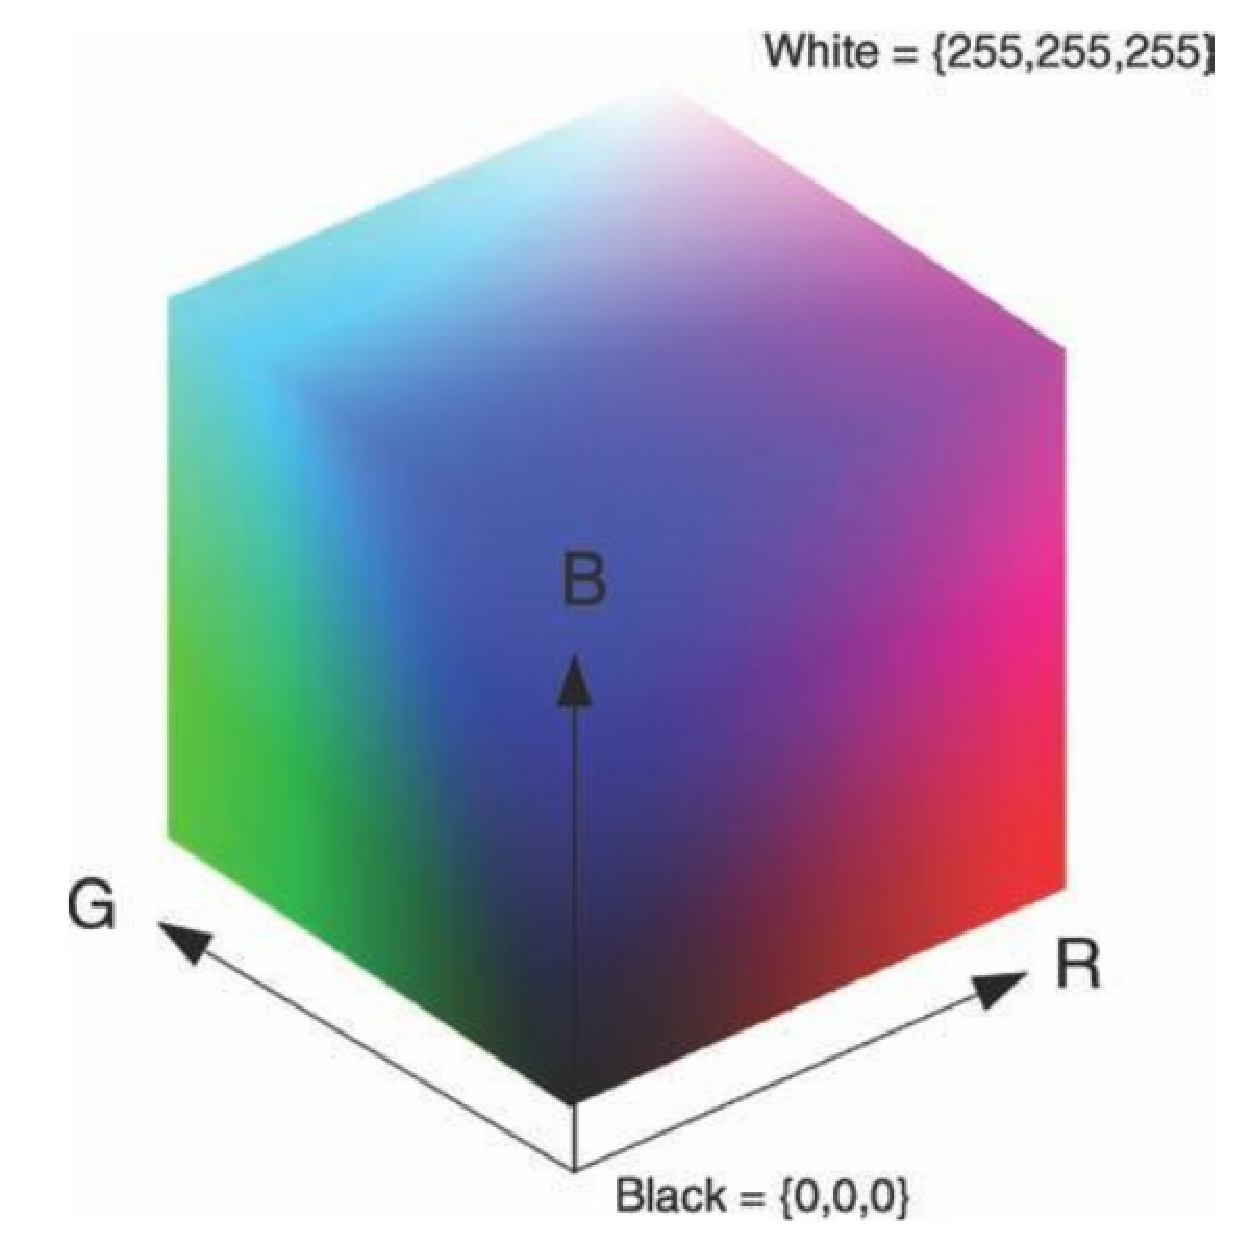
\includegraphics[scale=0.45]{images/rgb_cube}

\caption{A representation of the 3d RGB cube\cite{ChrisSolomon2011}}

\end{figure}

The main problem with the RGB-colorspace in image processing is its
non-linearity. Moving in a certain way in the cube might not produce
a color that is perceptually consistent with the change in each of
the channels.

The HSV-color space is closer to the human idea of color, because
it is easier to think of a color in terms of H(ue), S(aturation) and
V(alue). The value determines the brightness. The color space can
be represented in a 3d-hexagone, where the central vertical axis represents
the Intensity. Hue is defined as an angle in the range $[0,2\pi]$
and Saturation is the depth or purity of the color, it is measured
as a radial distance from the central axis\cite{Sural}.

The HSV-color space is advantageous in comparison to the RGB-color
space in color based image segmentation, because image objects are
more consistently contained in the resulting hue field than in the
channels of the RGB representation. This applies in particular to
changing light conditions\cite{ChrisSolomon2011}.

\begin{figure}[H]
\centering

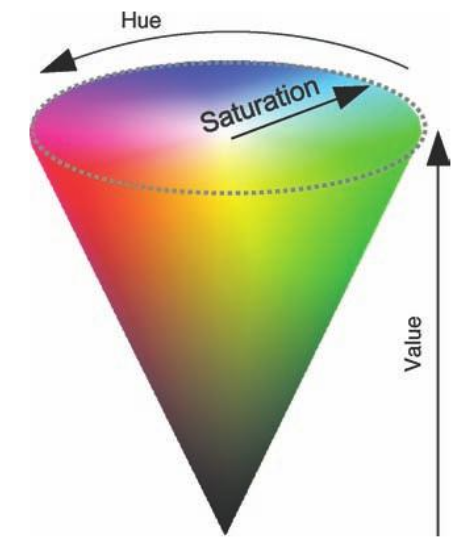
\includegraphics[scale=0.45]{/home/nilus/Dokumente/LyxBachelorarbeit/Bachelorarbeit/images/hsv_representation}

\caption{A representation of the HSV colorspace cone\cite{ChrisSolomon2011}}
\end{figure}

Both RGB and HSV spaces are however, not perceptually uniform; the
distances among colors perceived by the human are not mirrored by
similar distances between the points representing those colors in
such spaces\cite{Lucchese_colorimage}.

\chapter{Adaptive K-means clustering}

One of the logical extensions of the k-means algorithm used for color
segmentation seems to implement the algorithm not only on images,
but on whole video sequences. The existing algorithms for determining
the optimal cluster count could be transferred on whole videos, by
simply processing them frame by frame. Usually the resulting processing
time would prove unfit for most practical use if the algorithm is
applied on each frame of the video. While the regular k-means computing
time is feasible, at least if an iteration limit is implemented, the
computing time for dynamic cluster count identification as discussed
in 2.4 is tremendous, due to the repeated use of the basic k-means
algorithm. 

Hence, the first task of this bachelor thesis is to find a way to
adapt the identification of the optimal cluster number from images
to video sequences. 

Without further investigation the resulting cluster have only a limited
application use and can only represent the gathered knowledge of a
single frame. In order to include the information of the whole video
it is necessary to compare the resulting clusters of each frame. A
continuous occurring in several frames should eventually be recognized. 

Thus, the second task of this bachelor thesis is to implement a similarity
measurement for clusters to merge them over several frames. In order
to distinguish the clusters which are calculated using the k-means
algorithm in a single image and the clusters which are generated through
merging clusters of a video sequence, the latter kind will be referred
to as ``super-clusters''. 

\section{Dynamic cluster count algorithm in video sequences}

Due to color segmentation in video sequences and images being essentially
the same problem, the proposed algorithm by Siddheswar Ray and Rose
H. Turi, would also work in videos\cite{Ray1999} .Due to the assumption
that we are only looking at continuous video sequences, calculating
the optimal cluster count for each frame individually, without including
any knowledge gained from the previous calculations, would result
in redundant calculations for most videos. Thus the aim is to reduce
the calcuation time, while maintaining the same results algorithm
2.2 would produce if applied on each frame individually.

Often the optimal cluster count will be unchanged from one frame to
the subsequent one. The resulting cluster will only vary slightly,
either due to an occurred movement or due to a change of the lightning
condition. Hence it seems reasonable to look for an effective way
to include the gained knowledge of the previous frames. One option
would be to check whether cluster centers of the previous frame could
be kept as initial center for the k-means algorithm of the current
frame. 

As described in 2.3 the measure to evaluate the number of clusters
is the validity, its optimal value always falls on a local minimum
in comparison to a higher/lower cluster count. Which means that if
the cluster centers of the previous frame still constitute a local
minima in the current frame it is likely that the optimal cluster
count is unchanged. 

Unfortunately there are two major problems with this conclusion. Even
if the old cluster centers constitute a local minimum on the current
frame it is not guaranteed that it is the optimal solution. As described
in 2.3 the optimal cluster count for a synthetic image seems to be
the global minima and in case of a real image it would be the smallest
validity after the first local maxima. Neither for synthetic images,
nor for natural images can be checked whether the current minimum
constitutes the optimum without calculating the validity for each
k. 

Consider for example the validity chart in Fig 3.1. Searching for
the minimal validity would result in only 2 clusters. As discussed
in 2.3 the best validity in natural images would be at k = 8, because
it is the minmal value after the first local maximum. But if the previous
frame would have had 13 clusters, the adapted algorithm would continue
to work with those clusters, because k = 13 constitutes a local minimum.

\begin{figure}[H]
\centering

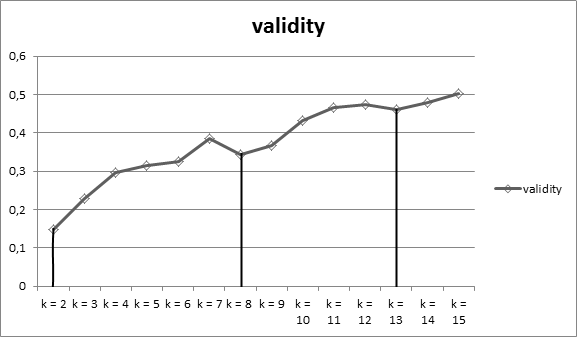
\includegraphics[scale=0.65]{/home/nilus/Dokumente/LyxBachelorarbeit/Bachelorarbeit/images/graph_validity}

\caption{Example of a validity chart}
\end{figure}

Even if the optimal number of clusters in a frame would equal the
used number of clusters in a former one, the old cluster centers might
be unfit as initialization points for k-means clustering in the current
frame. To get a good initialization point, the algorithm of Siddheswar
Ray and Rose H. Turi puts the whole image into a single cluster at
first. The mean of each pixel builds its cluster center. Continually
the cluster with the highest variance is split into two parts. Thus
using the old cluster centers as initialization points for k-means
clustering implies the assumption, that each time a cluster had the
highest variance in the previous frame, the same cluster would have
the highest variance in the current frame as well. 

Despite the occurring problems, using the local minima assumption
seems to be a good indicator to either keep the old cluster centers
as initialization points or start all over. The stated problems are
expected to occure rarely, due to mostly small occurring changes when
transitioning from one frame to another. The impact of identifying
the wrong cluster count in a video sequence will be further discussed
in the evaluation of this algorithm.\footnote{see 4.4 implementation in a video sequence}

At the beginning of this algorithm, the normal algorithm 2.2 will
be used on the first frame to get a good starting point to cluster
the remaining frames. In each iteration of algorithm 2.2 the cluster
centers for the current k have to be saved (line 2). This is necessary
in order to check whether the old cluster centers still constitutes
a local minima in the validity chart on the next frame. First the
validity of the best cluster centers in the first frame has to be
calculated on the current frame (line 4). As in all following steps
as well, the adapted cluster centers for k have to be stored (line
5). To check whether this validity constitutes a local minimum, the
validity for k+1 and k-1 is needed. To get this for k+1 the same process
as previously described can be used and the cluster with the highest
variance will be split (line 6). Afterwards the basic k-means algorithm
is applied and the validity is calculated (line 7).\footnote{see 2.3 Optimal cluster count}
Unfortunately it is not possible to simply remerge two clusters, because
there is no similar indicator as the variance for splitting, which
defines the clusters who have previously belonged together. Instead
for getting the validity for k-1 the corresponding cluster centers
of the previous cycle has to be used as initialization point for k-means
clustering (line 9), although this cluster centers have been generated
using a previous frame. Therefore it is important to save all calculated
cluster centers, because they might be used later. After running k-means
clustering and calculating the variance it can finally be checked,
if the validity for k consitutes a minimum (line 12).

If this is the case the described steps can simply be repeated on
the next frame. Otherwise the old cluster center seem to be unoptimal
and thus the whole algorithm 2.2 will be repeated on the current frame
(line 15).

\begin{algorithm}[H]
\begin{algorithmic}[1]
\State {Split the video sequence into frames} 
\State {Use algorithm 2.2 to find the optimal k for the first frame and save the cluster centers for each number of clusters}
\Repeat{ for each frame}
\State {Use standard k-means with existing cluster centers of k and calculate the validity}
\State {Save the new cluster centers for k}
\State {Split the cluster with the highest variance}
\State {Use the k-means algorithm and calculate the validity for k+1}
\State {Save the new cluster centers for k+1}
\State {Get the cluster centers of k-1 of the previously stored iterations}
\State {Use the k-means algorithm and calculate validity for k-1}
\State {Save the new cluster centers for k-1}
\If {validity of k-1 > validity of k <= validity of k+1}
\State { \textbf{continue} }
\Else 
\State {Use algorithm 2.2 and save the cluster centers for each number of clusters}
\EndIf
\Until {all frames are processed}
\State {Group the clusters into super-clusters according to a similarity measurement}
\end{algorithmic}

\caption{The adapted algorithm to find the optimal cluster count in video sequences}
\end{algorithm}

This algorithm will save computational time in cost of accuracy. In
some special cases it will provide non optimal solutions, this will
further be outlined in chapter 4. 

\section{Similarity measurement of clusters occurring over several frames}

In order to find a suitable similarity measurement for comparing clusters,
it is important to keep track of the goal. The fusion of several similar
clusters into one super-cluster should finally provide information
of the whole video. The basic k-means color segmentation algorithm
as described in 2.2 is repeatedly used in 2.3, would ultimately provide
only minimal information via the cluster centers. 

For example, if only the Euclidean distance of each cluster center
would be compared and the most similar ones would be merged, the gained
information could be seen as color histogram of the whole video sequence.
One improvement step is not only to include the color spaces, but
also the size to compare clusters. Thus clusters which share a color
with another cluster center but are ultimately unconnected, might
already be separated and don't share the same super-cluster. 

Without including the coordinates in any way, clusters cannot include
any information about shape and may contain disjointed areas. For
example in Figure 3.2 the optimal cluster count so far would be determined
as 2, because it only consists of 2 colors and a pure color segmentation
algorithm is applied. One cluster contains the black background and
the second one the red rectangles. To split clusters not only according
to their color, but also according to their geometrical distinctness,
the coordinates of each pixel need to be considered when calculating
the clusters. If the geomatrical distinctness is considered, the optimal
clustercount in Figure 3.2 changes from 2 to 3, because the rectangles
are not connected.

There are several ways to include geometrical features, but it would
be optimal if reasonable results could be achieved with the k-means
clustering algorithm itself. The basic idea hereby is to extend the
feature space from a 3d-vector which includes the color space, to
a 5d-vector which also includes the XY-coordinates. 

\begin{figure}[H]
\begin{center}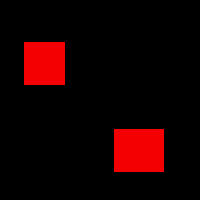
\includegraphics{images/beispiel}\end{center}\caption{Example of an image with optimal cluster count of 2 on pure color
segmentation and optimal cluster count of 3 when including geomatrical
features}
\end{figure}
A different approach to include geometrical knowledge is to detect
shapes in the already separated clusters, created by the k-means color
segmentation algorithm. The OpenCV library\cite{openCV_doc} already
implements the necessary functions for doing so. First a canny algorithm
will detect the edges of the respective cluster, before the openCV
method ``findContours(...)'' will finally try to calculate the corresponding
contours. Contours can be seen as boundaries, and in contrast to edges
they form closed curvatures. If there are several contours convoluted
in each other as for example seen in Figure 3.3, only the most outer
one is relevant and will represent a cluster. In the case of the image
in Figure 3.3 the only relevant contours are labeled from 0-2, because
the remaining contours are all enclosed in contour 2. 

\begin{figure}[H]
\begin{center}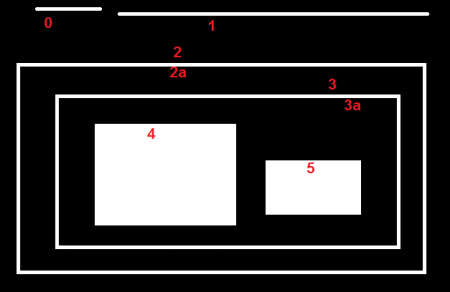
\includegraphics[scale=0.7]{images/hierarchy}

\caption{Example for hierachy in edge detection\cite{openCV_doc_hiearch}}

\end{center}
\end{figure}


\chapter{Results and Evaluation}

\section{Evaluation of the optimal cluster count}

\subsection{On synthetic images}

The results reported from Siddheswar Ray and Rose H. Turi \cite{Ray1999}
on synthetic images described in 2.3, could mostly be verified. On
very simple images as seen in Fig 4.1 the automatically specified
cluster count matches the actual used colors. Notice that this section
is only concerned about color segmentation.

\begin{figure}[H]
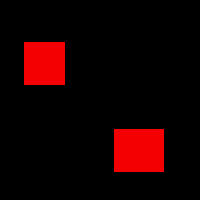
\includegraphics[scale=0.75]{images/beispiel}~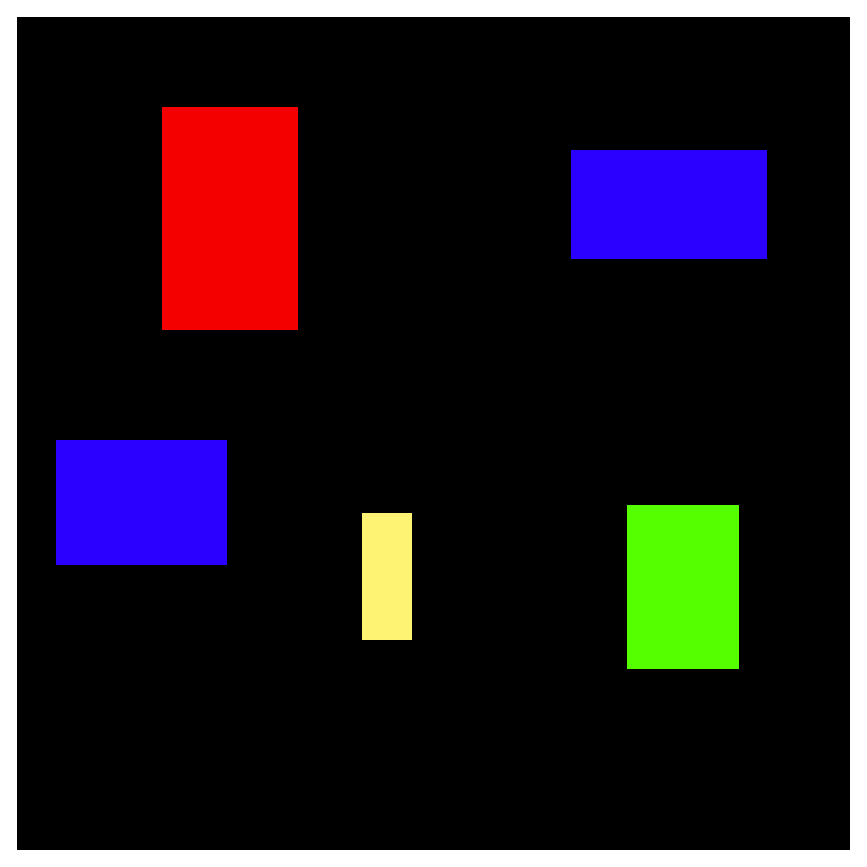
\includegraphics[scale=0.375]{images/beispiel2}~
\includegraphics{images/beispiel3}\caption{Simple generated images with known used number of colours (2, 5, 4)}
\end{figure}

Surprisingly the calculated optimal cluster count using the RGB color
space and a maximal cluster count of 25 in Figure 4.2 was determined
as 10 instead of the expected 5 clusters. This error occurs due to
the different numbers of colors used in differing shapes. Each rectangle
consists of only of one specific color, whereas the circle can be
distinguished into several RGB-values. The core of the circle and
everything in close distance has only one color value, but the closer
the distance to the boundary the more the color changes in order to
achieve an effect of anti-aliasing, this can be seen in Figure 4.3.
Anti-aliasing makes the rectangle shape of pixels on a computer display
less visible for the human eye. In this specific case the circle consists
of 49 different RGB values. Due to the relationship of inter cluster
distance and intra cluster distance the circle is split into 5 different
clusters. The conversion into HSV did not result in a calculated cluster
count of 5 either; instead it went up to 13 (keeping the Euclidean
distance as distance measurement). As described in 2.4 the different
nature of the RGB color space and HSV color space results in different
distances in between colors. Many of the 49 RGB colors will probably
share the same hue value, but can be further clustered according to
the saturation and brightness. Therefore this results in different
clusters in comparison to the RGB color space and with it to a rise
of the calculated optimal cluster count.

Given that the used colors in a natural images are expected to be
a lot more than 53, the performed clustering will never be on a comparable
fine level. The decrease of the intra cluster distance would lead
to a lower inter cluster distance and supposedly the validity would
increase.

\begin{figure}[H]
\begin{subfigure}[c]{0.3\textwidth} 
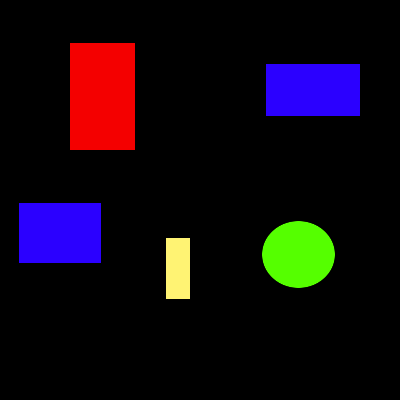
\includegraphics[width=1\textwidth]
{images/circle.png} 
\subcaption{Source image} 
\end{subfigure}
\begin{subfigure}[c]{0.3\textwidth} 
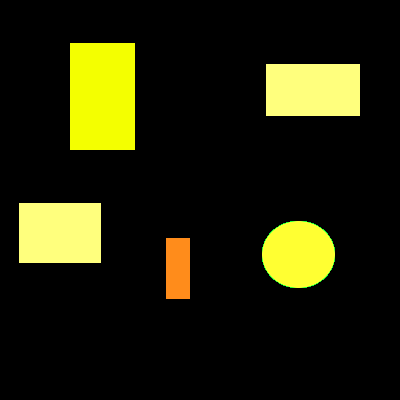
\includegraphics[width=\textwidth]{images/circle_HSV.png} 
\subcaption{converted into HSV} 
\end{subfigure}
\begin{subfigure}[c]{0.3\textwidth} 

\includegraphics[width=\textwidth]{images/circle_anti_aliasing.png} 
\subcaption{zoomed in circle} 
\end{subfigure}

\caption{Simple generated image including a circle converted into HSV}
\end{figure}

Increasing the number of circles and adding more colors overall to
testing images as for example seen in Figure 4.3, resulted in a correct
computation of the cluster count in RGB color space. The particular
image is built of 4564 RGB values and the right cluster count of 10
is calculated. Transferring this image into the HSV color space resulted
in the computation of 10 as well. 

\begin{figure}[H]
\begin{subfigure}[c]{0.3\textwidth} 
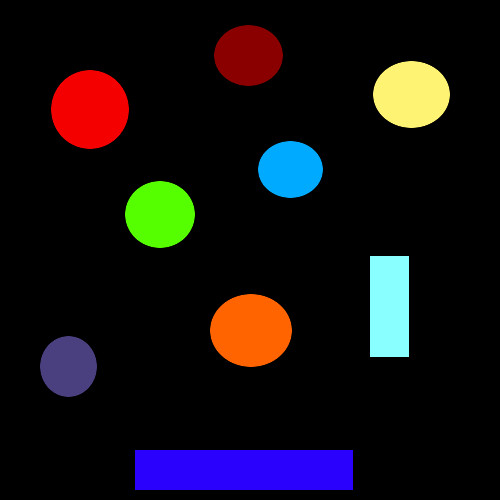
\includegraphics[width=1\textwidth]
{images/4564colors.jpg} 
\subcaption{Source image} 
\end{subfigure}
\begin{subfigure}[c]{0.3\textwidth} 
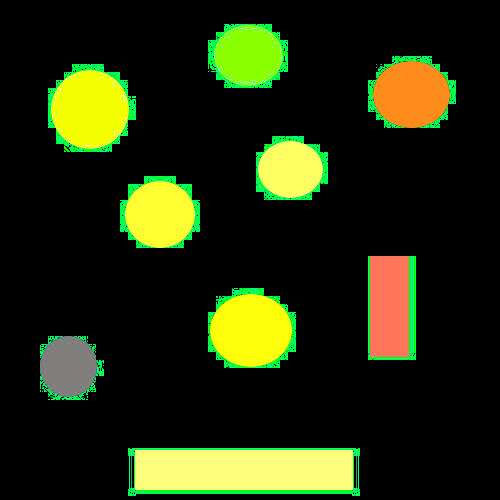
\includegraphics[width=\textwidth]{images/colors_to_HSV.png} 
\subcaption{clustered in HSV} 
\end{subfigure}
\begin{subfigure}[c]{0.3\textwidth} 
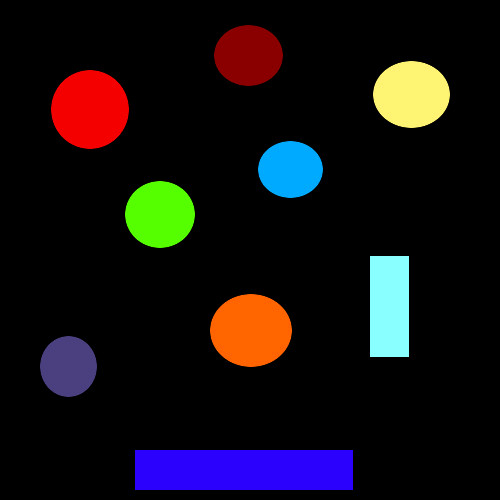
\includegraphics[width=\textwidth]{images/colors_toHSV2BGR.png} 
\subcaption{b) converted into RGB} 
\end{subfigure}\caption{Simple generated image build of 4564 RGB values converted into HSV}
\end{figure}


\subsection{On real images}

Until now the cluster count was only tested on self-generated images
with known optimal cluster count. On real images this is usually only
roughly estimable.

The algorithm was tested clustering images of the Berkeley Segmentation
Dataset\cite{Arbelaez2011} and provided satisfactory results. To
evaluate the dynamic cluster count the clustered images, were compared
to the images generated with a higher/lower number of clusters. These
are also generated with algorithm 2.2. It increments the number of
clusters succesively until $k_{\max}$ is reached, hence the images
in the range from k = 2 to k = $k_{\max}$can be used for comparison
purposes.

\begin{figure}[H]
\begin{subfigure}[c]{0.5\textwidth}
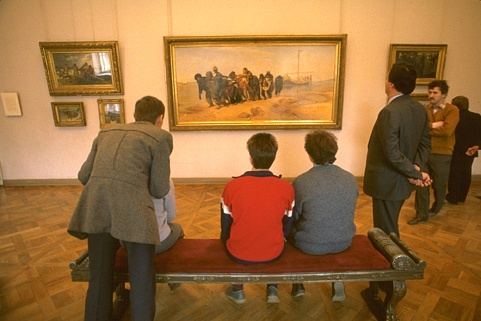
\includegraphics[width=1\textwidth]{images/128035.jpg} 
\subcaption{Source image}
\end{subfigure}
\begin{subfigure}[c]{0.5\textwidth} 
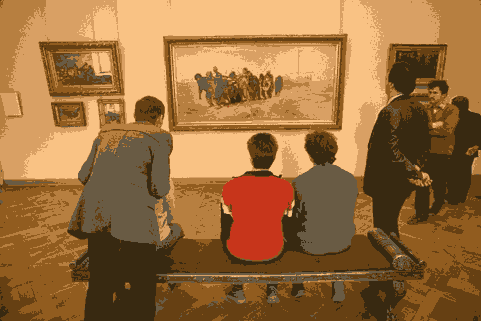
\includegraphics[width=1\textwidth]
{/home/nilus/Dokumente/LyxBachelorarbeit/Bachelorarbeit/images/128035_rgb_8_optimal.png} 
\subcaption{calculated k = 8} 
\end{subfigure}
\begin{subfigure}[c]{0.5\textwidth} 
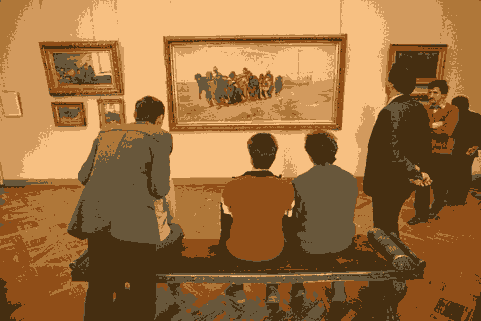
\includegraphics[width=\textwidth]{/home/nilus/Dokumente/LyxBachelorarbeit/Bachelorarbeit/images/128035_rgb_6.png} 
\subcaption{k = 6} 
\end{subfigure}
\begin{subfigure}[c]{0.5\textwidth} 
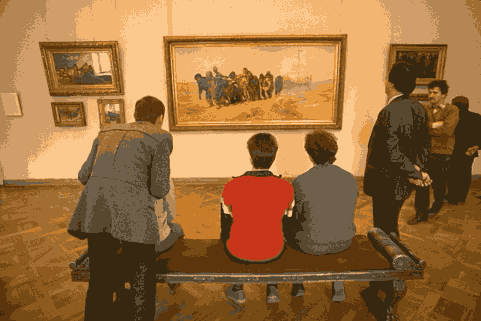
\includegraphics[width=1\textwidth]
{/home/nilus/Dokumente/LyxBachelorarbeit/Bachelorarbeit/images/128035_rgb_14.png} 
\subcaption{k = 14} 
\end{subfigure}\caption{Gallery example from the Berkeley Database clustered in RGB-color
space}
\end{figure}

The calculated cluster count of 8 in Figure 4.4 is the first cluster
count where, the red shirt builds its own cluster. It seems as in
a smaller cluster counts the inter cluster distance is bigger. In
k > 8 the intra cluster distance seems to be minimized but has only
minimal visible impact, because of the higher inter cluster distance
before. Thus k = 8 seem to be the right choice. 

\begin{figure}[H]
\begin{subfigure}[c]{0.5\textwidth}
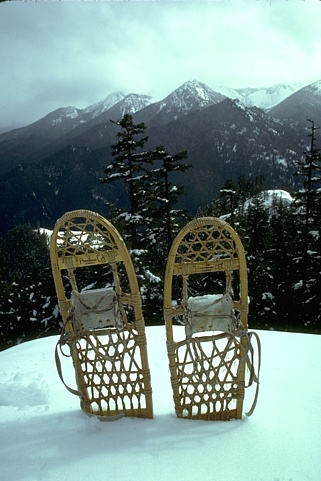
\includegraphics[width=1\textwidth]{/home/nilus/Dokumente/LyxBachelorarbeit/Bachelorarbeit/images/2018.jpg} 
\subcaption{Source image}
\end{subfigure}
\begin{subfigure}[c]{0.5\textwidth} 
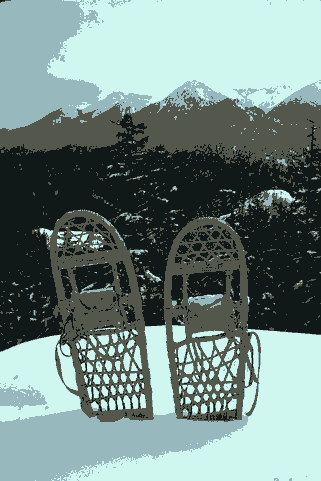
\includegraphics[width=1\textwidth]{/home/nilus/Dokumente/LyxBachelorarbeit/Bachelorarbeit/images/2018_rgb_4_optimal.png} 
\subcaption{calculated k = 4} 
\end{subfigure}
\begin{subfigure}[c]{0.5\textwidth} 
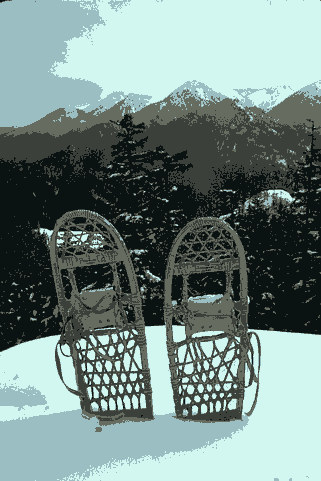
\includegraphics[width=\textwidth]{/home/nilus/Dokumente/LyxBachelorarbeit/Bachelorarbeit/images/2018_rgb_5.png} 
\subcaption{k = 5} 
\end{subfigure}
\begin{subfigure}[c]{0.5\textwidth} 
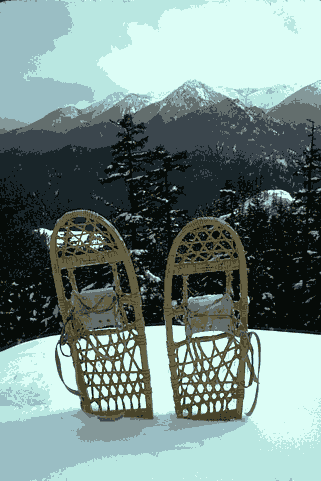
\includegraphics[width=1\textwidth]{/home/nilus/Dokumente/LyxBachelorarbeit/Bachelorarbeit/images/2018_rgb_10.png} 
\subcaption{k = 10} 
\end{subfigure}

\caption{Snow shoes example from the Berkeley Database clustered in RGB-color
space}
\end{figure}

The calculated cluster count of 4 in Figure 4.5 seems to retain most
key features of the image, the results seen in c) for k=3 seem to
be similarly well. The cluster count of 10 seen in d) might be preferable
due to the existence of a cluster solely for the snow shoes. The latter
impression probably arises of our focus on the image center; but looking
at the sky reveals that it has already been segmented into 3 sections
at this point. 

\begin{figure}[H]
\begin{subfigure}[c]{0.5\textwidth}
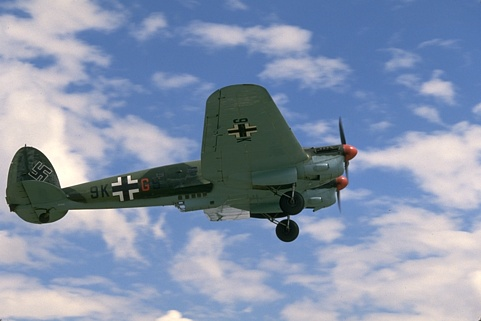
\includegraphics[width=1\textwidth]{/home/nilus/Dokumente/LyxBachelorarbeit/Bachelorarbeit/images/3063.jpg} 
\subcaption{Source image}
\end{subfigure}
\begin{subfigure}[c]{0.5\textwidth} 
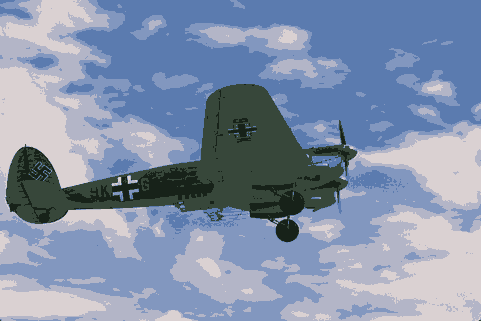
\includegraphics[width=1\textwidth]
{/home/nilus/Dokumente/LyxBachelorarbeit/Bachelorarbeit/images/3063_rgb_6_optimal.png} 
\subcaption{calculated k = 6} 
\end{subfigure}
\begin{subfigure}[c]{0.5\textwidth} 
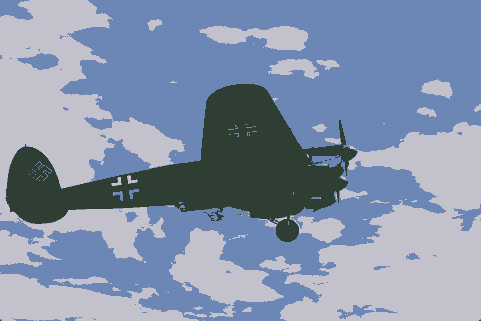
\includegraphics[width=\textwidth]{/home/nilus/Dokumente/LyxBachelorarbeit/Bachelorarbeit/images/3063_rgb_3.png} 
\subcaption{k = 3} 
\end{subfigure}
\begin{subfigure}[c]{0.5\textwidth} 
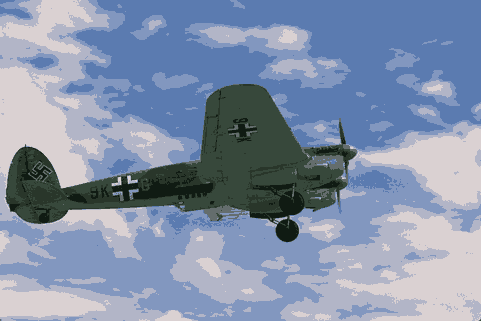
\includegraphics[width=1\textwidth]
{/home/nilus/Dokumente/LyxBachelorarbeit/Bachelorarbeit/images/3063_rgb_8.png} 
\subcaption{k = 8} 
\end{subfigure}

\caption{Airplane example from the Berkeley Database clustered in RGB-color
space}
\end{figure}

The calculated optimal cluster count of 6 in Figure 4.6 seems to be
the most adequate cluster number, although k=3 seems to highlight
the plane better. However, k-means clustering is an unsupervised algorithm
without prior knowledge, hence the cluster count of 6 retains more
information of the background as well.

Using the HSV-color space instead of the RGB-color space did not lead
to considerably better results. Strikingly the calculated optimal
cluster count was mostly higher in HSV as for example seen in Figure
4.7. Otherwise the same findings as in the RGB-color space could be
made. Overall the comparison did not favor any color space. The results
were subjectively examined on the same level. The determination of
which color space to use, should depend on the final task of the clustering
algorithm. Because the following work is rather on an abstract level
than on implementing the algorithm on a particular task and because
the underlying algorithm for determining the cluster count was originally
proposed for the RGB color space, the latter one will be used in the
evaluation of the dynamic cluster count on video sequences. 

\begin{figure}[H]
\begin{subfigure}[c]{0.5\textwidth}
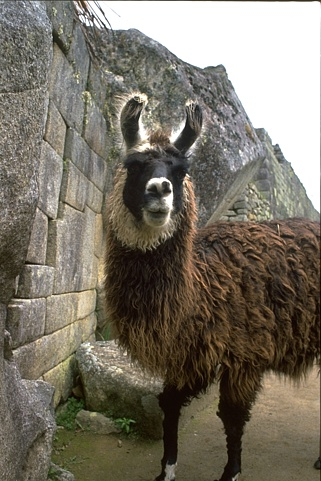
\includegraphics[width=0.5\textwidth]{/home/nilus/Dokumente/LyxBachelorarbeit/Bachelorarbeit/images/6046.jpg} 
\subcaption{Source image}
\end{subfigure}
\begin{subfigure}[c]{0.5\textwidth} 
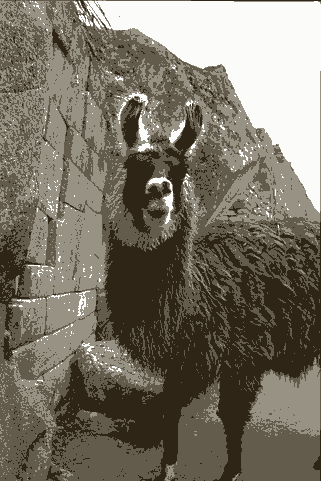
\includegraphics[width=0.5\textwidth]
{/home/nilus/Dokumente/LyxBachelorarbeit/Bachelorarbeit/images/6046_rgb_4.png} 
\subcaption{calculated k = 4 (RGB)} 
\end{subfigure}
\begin{subfigure}[c]{0.5\textwidth} 
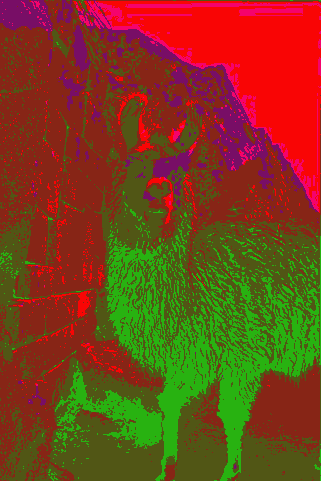
\includegraphics[width=0.5\textwidth]{/home/nilus/Dokumente/LyxBachelorarbeit/Bachelorarbeit/images/6046_hsv_6.png} 
\subcaption{calculated k = 6 (HSV)} 
\end{subfigure}
\begin{subfigure}[c]{0.5\textwidth} 
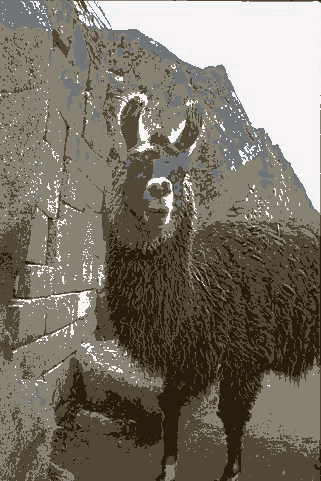
\includegraphics[width=0.5\textwidth]
{/home/nilus/Dokumente/LyxBachelorarbeit/Bachelorarbeit/images/6046_hsv_6_to_rgb.png} 
\subcaption{c) converted into RGB} 
\end{subfigure}

\caption{Comparison of results in RGB and HSV color spaces}
\end{figure}


\section{Implementation in a video sequence}

\subsection{On synthetic video sequences}

Implementing the dynamical cluster count as described in algorithm
3.1 into a simple synthetic video sequence revealed that the cluster
count incremented correctly when necessary, but failed to detect required
reductions of k.

Figure 4.8 shows an example of a video sequence. In image a) to d)
the cluster count stays the same and is recognized correctly. The
new appearance of a rectangle in cluster e) leads to a new cluster
count calculation. In cluster g) the green rectangle is gone and a
new cluster count calculation should be the result. Unfortunately
the algorithm fails to identify the change and keeps the old cluster
count. 

\begin{figure}[H]
\begin{subfigure}[c]{0.22\textwidth}
\frame {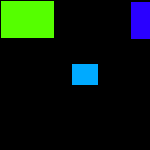
\includegraphics[width=1\textwidth]
{images/simple_VidExample0.png}}
\subcaption{k = 3}
\end{subfigure}
\begin{subfigure}[c]{0.22\textwidth}
\frame {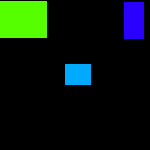
\includegraphics[width=1\textwidth]
{images/simple_VidExample1.png}}
\subcaption{k = 3}
\end{subfigure}
\begin{subfigure}[c]{0.22\textwidth}
\frame {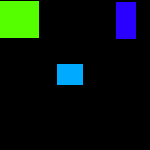
\includegraphics[width=1\textwidth]
{images/simple_VidExample2.png}}
\subcaption{k = 3}
\end{subfigure}
\begin{subfigure}[c]{0.22\textwidth}
\frame {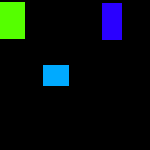
\includegraphics[width=1\textwidth]
{images/simple_VidExample3.png}}
\subcaption{k = 3}
\end{subfigure}
\begin{subfigure}[c]{0.325\textwidth}
\frame {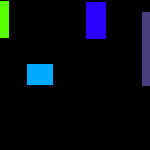
\includegraphics[width=0.67\textwidth]
{images/simple_VidExample4.png}}
\subcaption{k = 4}
\end{subfigure}
\begin{subfigure}[c]{0.325\textwidth}
\frame {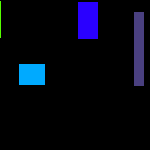
\includegraphics[width=0.67\textwidth]
{images/simple_VidExample5.png}}
\subcaption{k = 4}
\end{subfigure}
\begin{subfigure}[c]{0.325\textwidth}
\frame {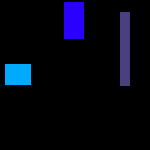
\includegraphics[width=0.67\textwidth]
{images/simple_VidExample6.png}}
\subcaption{k = 3}
\end{subfigure}

\caption{\foreignlanguage{ngerman}{A simple video sequence in which areas are moving out of the video}}
\end{figure}

This and similar tests showed that as long as something is added to
the scene, the variance calculation of previous runs for determining
the cluster count will still be meaningful for the current frame.
If the clusters are calculated with k-means using the cluster centers
of the previous frame as initialization points, the generated clusters
will have a higher variance if a new area is added to the scene. Thus
the validity measure will usually decrease if the number of clusters
is increased, this is the same principle used in algorithm 2.2. Even
if the algorithm for identifying the optimal cluster count would have
split clusters in a different way if run on the current image, the
disparity can still be regulated. For the transformation from k to
k+1, the k-means algorithm splits the cluster with the highest variance
on the current image. In contrast the initialization points for k-1
are solely received via the calculation on previous frames. Therefore
the calculations of the validity for k-1 needs to be improved. One
possibility for doing so is to use the same procedure as k+1 received
already. Instead of calculating the validity for k-1 immediately,
the cluster centers for k-2 (if k>3) will be used as initialization
points. The new clusters will be split once again as described in
2.3 and the arising cluster centers will be used to calculate the
validity for k-1. Another improvement can be achieved, when the order
of the validity checks is changed. The validity for k-1 will be checked
first, the generated clusters will be split twice and used to calculate
the validity for k and k+1.

With this slight modification the algorithm achieved the right cluster
count results on all self-generated simple video sequences similar
to Figure 4.8 as long as the conditions remained constant. The considered
cases included appearing and disappearing areas both solely and simultaneously. 

However, adding blurring, noise or light effects to an image resulted
most often in a different cluster count than before, indicating unstableness
in real images on changing conditions. But the impact of these effects
on simple images with only few features is found to be stronger and
less subtle than in most real occurring condition changes seen in
natural video sequences.

To actually compare the produced cluster centers over several frames,
the generated cluster centers of the first frame were used as the
first centers of ``super-clusters'' (=merged clusters of frames).
On each iteration of the algorithm, after the optimal number of clusters
has been identified, the new cluster centers are compared to the centers
of existing super-clusters. For comparison the usual Euclidean color
space distance and the Euclidean distance of the coordinate centers
of the cluster centers and the super-clusters were calculated. In
order to add them, they had to be normalized.

\[
d_{color}=|v_{color\,1}-v_{color\,2}|
\]

\[
d_{coord}=|v_{coord\,1}-v_{coord\,2}|
\]

\[
d_{v1\,v2}=d_{color}+d_{coord}
\]

With $v_{1}$ being the normalized cluster center and $v_{2}$ being
the normalized center of the super-cluster. $v_{color}$ only includes
the color information and $v_{coord}$ only includes the center coordinates.

If the sum of both distances of the closest super-cluster was smaller
than a self-determined $\delta_{dis}$ the cluster center belonged
to the super-center. 

\[
d_{v1\,v2}<d_{max\cdot\delta}=\delta_{dis}
\]
In this case the center of the super-cluster had to be updated. Thus
the old center of the super-cluster is simply replaced with the newest
member. To get to a good $\delta_{dis}$ the maximal possible distance
has to be considered and scaled accordingly. An alternative approach
is to add the center of the cluster to the center of the super-cluster
and divide it by 2. This led to more stable results. As soon as one
outlier appears the center is shifted in the wrong direction. Because
it is likely that new clusters will not be assigned to the right super-cluster.
Normally we expect clusters to move continuously in the same direction,
hence the first method led mostly to better results.

Otherwise if the distance to the closest super-cluster was bigger
than $\delta_{dis}$ the cluster center is not part of an existing
supercluster and its values will be the initial values of a new super-cluster.

This method generated the right results for simple synthetic video
sequences using a reasonable $\delta$. For example, the video sequence
seen in Fig 4.8 $\sim0.06<\delta<0.6$ produced right results. Overall
$\delta=0.15$ was found to be a good threshold, a higher value for
$\delta$ often resulted in putting several clusters of one frame
into a single super-cluster.

\subsection{On real video sequences}

To evaluate the performace of algorithm 3.1 its calculated adaptive
cluster count was compared to the outcome produced by its predecessor
algorithm developed by Ray and Rose H. Turi\footnote{algorithm 2.2},
where each frame was processed individually. This was done on video
sequences of the Freiburg-Berkeley Motion Segmentation Dataset\cite{Ochs2014},
one example consisting of only 19 frames can be seen in Figure 4.9.

The adapted and unadapted algorithms produced the same cluster count
on most frames, however, the adapted algorithm tended to switch the
cluster count less times than the unadapted one. This outcome had
to be expected, as described in 3.1 the adapted algorithm will not
change the cluster count if the validity currently constitutes a local
minima, whereas the unandapted algorithm will always go with the global
minima.

\begin{figure}[H]
\begin{center}
\frame{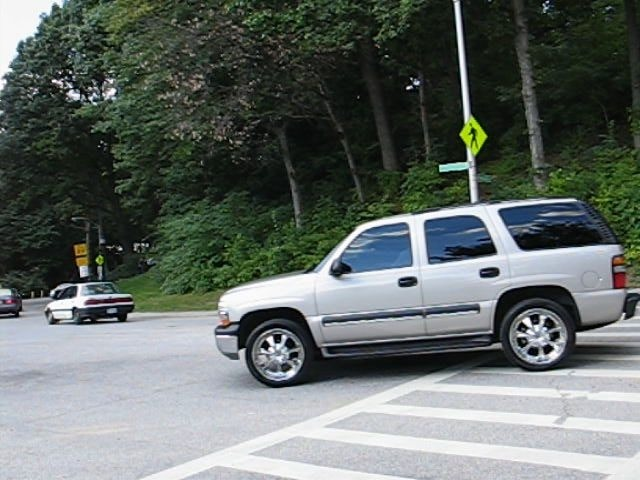
\includegraphics[width=0.22\textwidth]{images/cars1_01.jpg}}
\frame{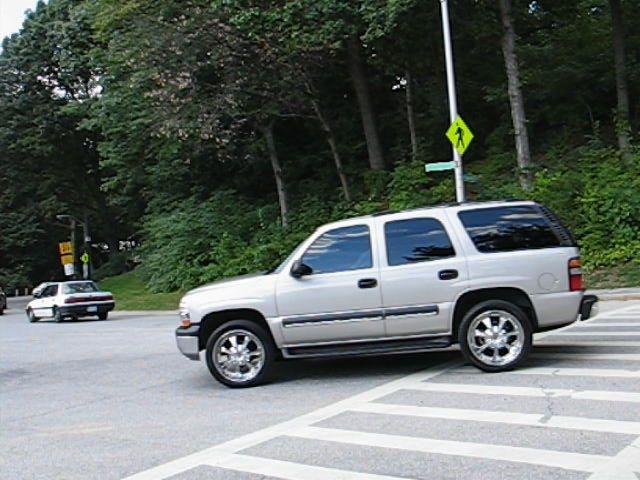
\includegraphics[width=0.22\textwidth]{images/cars1_02.jpg}} 
\frame{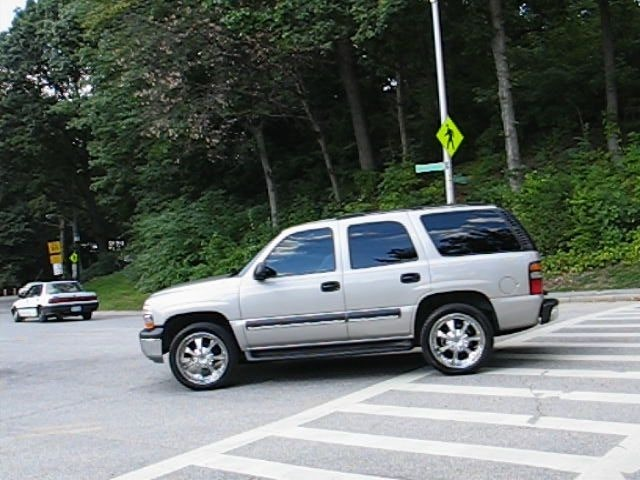
\includegraphics[width=0.22\textwidth]{images/cars1_03.jpg}}
\frame{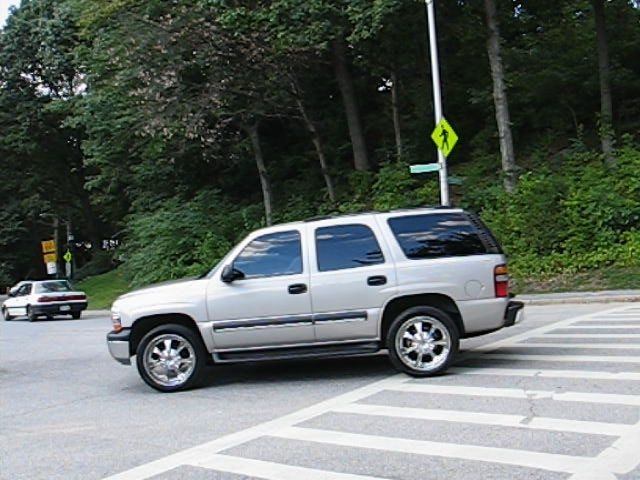
\includegraphics[width=0.22\textwidth]{images/cars1_04.jpg}}
\frame{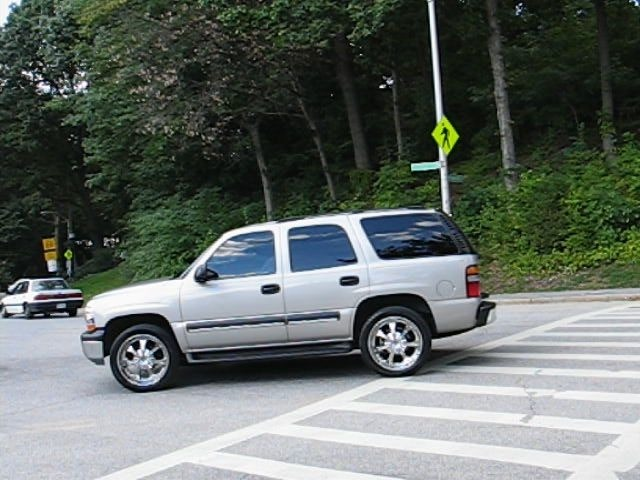
\includegraphics[width=0.22\textwidth]{images/cars1_05.jpg}} 
\frame{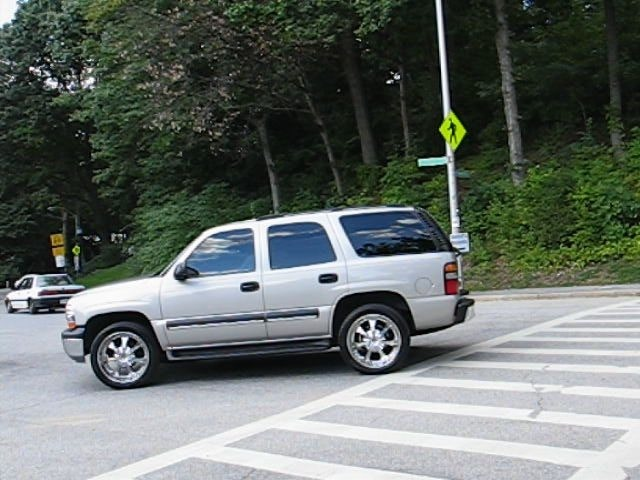
\includegraphics[width=0.22\textwidth]{images/cars1_06.jpg}}
\frame{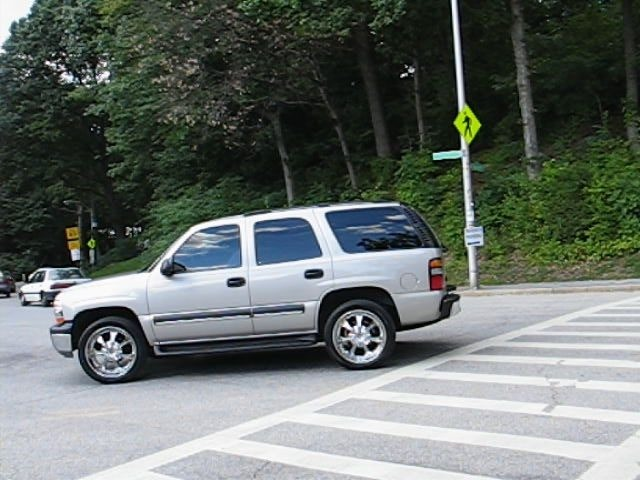
\includegraphics[width=0.22\textwidth]{images/cars1_07.jpg}}
\frame{\includegraphics[width=0.22\textwidth]{images/cars1_08.jpg}} 
\frame{\includegraphics[width=0.22\textwidth]{images/cars1_09.jpg}}
\frame{\includegraphics[width=0.22\textwidth]{images/cars1_10.jpg}}
\frame{\includegraphics[width=0.22\textwidth]{images/cars1_11.jpg}} 
\frame{\includegraphics[width=0.22\textwidth]{images/cars1_12.jpg}}
\frame{\includegraphics[width=0.22\textwidth]{images/cars1_13.jpg}}
\frame{\includegraphics[width=0.22\textwidth]{images/cars1_14.jpg}} 
\frame{\includegraphics[width=0.22\textwidth]{images/cars1_15.jpg}}
\frame{\includegraphics[width=0.22\textwidth]{images/cars1_16.jpg}}
\frame{\includegraphics[width=0.22\textwidth]{images/cars1_17.jpg}} 
\frame{\includegraphics[width=0.22\textwidth]{images/cars1_18.jpg}}
\frame{\includegraphics[width=0.22\textwidth]{images/cars1_19.jpg}}
\end{center}

\caption{Example of a video sequence used for evaluation}
\end{figure}

\selectlanguage{english}%
\begin{table}[H]
\centering 
\begin{subtable}{.5\textwidth} 
	\centering
	\begin{tabular}{ccl}
	\toprule
	Frame & k & super-clusters \\
	\midrule
	1-2 & 6 &  0 1 2 3 4 5 \\ 
	3-11 & 5 & 0 2 1 3 4 \\
	12-16 & 5 & 0 1 2 3 4 \\
	\rowcolor{LightCyan}17 & 6 & 0 3 2 4 1 5  \\
	\rowcolor{LightCyan}18-19 & 8 & 0 5 2 4 1 4 3 5\\
	\bottomrule
	& & 8 super-clusters
	\end{tabular} 
	\caption{results for Fig 4.9 using the unadapted  \mbox{algorithm}}
\end{subtable}%
\begin{subtable}{.5\textwidth} 
	\centering
	\begin{tabular}{ccl}
	\toprule
	Frame & k & super-clusters \\
	\midrule
	1-2 & 6 &  0 1 2 3 4 5 \\
	3-11 & 5 & 0 2 1 3 4 \\
	12-16 & 5 & 0 1 2 3 4 \\
	\rowcolor{LightCyan}17 & 5 & 0 1 2 3 4 \\
	\rowcolor{LightCyan}18-19 & 5 & 0 1 2 3 4 \\
	\bottomrule
	& & 7 super-clusters
	\end{tabular} 
	\caption{results for Fig 4.9 using the adapted  \mbox{algorithm}}
\end{subtable} 

\caption{\foreignlanguage{british}{The results produced on the video sequence of Figure 4.9 in RGB with
$\delta=0.2$}}
\end{table}

\selectlanguage{british}%
Table 4.1 shows the calculated number of clusters and the respective
super-clusters for the video sequence seen in Figure 4.9. The index
on the list of super-clusters corresponds to the cluster of each frame
which is assigned to the respective super-cluster. In this particular
case the adapted algorithm produced only in 3 out of 19 frames a different
outcome.

The different results produced in the adapted and unadapted algorithm
don't necessarily mean that the calculated cluster count of the adapted
algorithm is worse. Sometimes it might be reasonable to keep the cluster
count more stable. If the cluster count is mostly unchanged, the generated
clusters are more similar and thus merge into fewer super-clusters.
This might be useful for tracking the movement of an object. If the
object is recognized in one of the clusters of the first frame, the
corresponding super-cluster might ease the recognition in the following
clusters. Figure 4.10 for example shows the super-cluster labeled
as 4 in Table 4.1, where most key features of the car are visible.

\begin{figure}[H]
\begin{center}
\frame{\includegraphics[width=0.22\textwidth]{images/4_0.png}}
\frame{\includegraphics[width=0.22\textwidth]{images/4_1.png}} 
\frame{\includegraphics[width=0.22\textwidth]{images/4_2.png}}
\frame{\includegraphics[width=0.22\textwidth]{images/4_3.png}} 
\frame{\includegraphics[width=0.22\textwidth]{images/4_4.png}}
\frame{\includegraphics[width=0.22\textwidth]{images/4_5.png}}
\frame{\includegraphics[width=0.22\textwidth]{images/4_6.png}} 
\frame{\includegraphics[width=0.22\textwidth]{images/4_7.png}} 
\frame{\includegraphics[width=0.22\textwidth]{images/4_8.png}} 
\frame{\includegraphics[width=0.22\textwidth]{images/4_9.png}} 
\frame{\includegraphics[width=0.22\textwidth]{images/4_10.png}} 
\frame{\includegraphics[width=0.22\textwidth]{images/4_11.png}}
\frame{\includegraphics[width=0.22\textwidth]{images/4_12.png}} 
\frame{\includegraphics[width=0.22\textwidth]{images/4_13.png}} 
\frame{\includegraphics[width=0.22\textwidth]{images/4_14.png}}
\frame{\includegraphics[width=0.22\textwidth]{images/4_15.png}} 
\frame{\includegraphics[width=0.22\textwidth]{images/4_15.png}} 
\frame{\includegraphics[width=0.22\textwidth]{images/4_17.png}} 
\frame{\includegraphics[width=0.22\textwidth]{images/4_18.png}} 
\end{center}\caption{The clusters, which are put into the super-cluster 4 in Table 4.1}

\end{figure}

However, it is unlikely that the features of an object are completely
put into one cluster.

The super-clusters could also be used to compress the data size of
the video sequence. The video sequence of Figure 4.9 could be encoded
to only 7 colors when using the adapted algorithm. For other purposes
it is hardly possible to rate the performance of this algorithm in
reference to the super-clusters, due to the lack of similar scientific
work. If the clusters would actually possess striking visual features
the super-clusters could be evaluated further. Therefore it makes
sense to try to include geometrical features into the segmentation
process.

\section{Evaluation of k-means clustering with a 5d-feature vector}

Using a 5d-feature vector, consisting of the color space and the coordinates
promises two main advantages. Clustered regions would be closer to
semantic knowledge, because regions with similar colors are already
split and thus the results are more useful for comparing clusters
over the cause of a video sequence. Furthermore after the k-means
algorithm has clustered each frame separately, the whole outcome can
build a new dataset, which then again could be clustered via k-means
to fuse the clusters of each frame into super-clusters holding information
of the whole video sequence. The requirement to do so are reliable
and reasonable generated results when clustering single images. 

To get reasonable images the 5d-feature vector has to be normalized
first.

\[
\text{5d-feature Vector: }\overrightarrow{v}=\begin{array}{c}
r\\
g\\
b\\
x\\
y
\end{array}
\]

\[
\overrightarrow{v}_{normalized}=\begin{array}{c}
\frac{r}{255}\frac{1}{3}\\
\frac{g}{255}\frac{1}{3}\\
\frac{b}{255}\frac{1}{3}\\
\frac{x}{\max X}\frac{1}{2}\alpha\\
\frac{y}{\max Y}\frac{1}{2}\alpha
\end{array}
\]

Where $\alpha$ is the scaling factor. Usually the color space will
be seen as more important than the geometric features, so $\alpha$
will be close to zero. 

The same normalization procedure should theoretically be applied on
the variance calculation as well. Unfortunately due to the incoherent
shape of the background, the cluster containing the background area
had often the highest variance out of the calculated clusters. Figure
4.11 shows an example of this occurrence; the white area represents
the not contained area of the specific cluster. While the algorithm
gets the expected result for k=2 and $\alpha=0.004$ (a ratio of 250:1),
it fails for k=3-5 and splits the background further.\footnote{Using the algorithm 2.2 to determine the optimal cluster count}

\begin{figure}[H]
\begin{subfigure}[c]{0.2\textwidth} 
\includegraphics[width=1\textwidth]
{/home/nilus/Dokumente/LyxBachelorarbeit/Bachelorarbeit/images/beispiel.png} 
\subcaption{source image} 
\end{subfigure}
\begin{subfigure}[c]{0.2\textwidth} 
\frame {\includegraphics[width=1\textwidth]
{images/beispiel_clusters.png}}
\subcaption{cluster 1} 
\end{subfigure}
\begin{subfigure}[c]{0.2\textwidth} 
\includegraphics[width=1\textwidth]
{images/beispiel_clusters2.png} 
\subcaption{cluster 2} 
\end{subfigure}
\begin{subfigure}[c]{0.2\textwidth} 
\includegraphics[width=1\textwidth]
{images/beispiel_clusters3.png} 
\subcaption{cluster 3} 
\end{subfigure}

\caption{Example of single clusters when splitting the wrong cluster using
a 5d-feature vector}
\end{figure}

Ignoring the geometrical features while calculating the variance lead
to better results in the case of Figure 4.11, but only by chance the
rectangles were the first cluster in k=2. In order to split the right
cluster a different measurement than the variance would be needed.
Even if the problem of finding the right cluster to split is ignored
and the right cluster is assigned manually, it didn't generate reasonable
results. The major problem hereby is to find a scale of the geometric
features to the color features. In some images this scale could be
found, but did not result in equally good clusters on different images.
The requirement to produce results on any image would be to assign
the scale dynamically to each image. But for some images there might
even exist no appropriate ratio of color features and geometrical
features, which would lead to meaningful clusters. A potential instance
of this will be further discussed in section 4.4. 

\section{Evaluation of the alternative approach}

Due to the inefficiency using a 5d-feature vector, especially with
the problem of getting a right measure for the optimal cluster count,
it seems easier to separate the splitting according to color features
and the splitting according to geometrical features into two processes.
Instead of clustering with a 5d-feature vector, the well performing
3d-vector including only the color space can be retained and each
cluster might be further divided. 

We only want to divide clusters with clear geometrical boundaries
further. Hence if it is possible to draw several polygons without
overlapping, where the area of the polygons is made up by the pixels
of the clusters, the polygons will build new clusters.

This can be achieved using the openCV library\cite{openCV_doc}.\footnote{see section 3.2}
Hereby one major problem needs to be considered. The cluster(s) which
hold the color information of the background might lead to the same
detected boundaries as the clusters which are actually surrounded
by the background.

\begin{figure}[H]
\begin{subfigure}[c]{0.2\textwidth}
\includegraphics[width=1\textwidth]
{images/beispiel.png} 
\subcaption{}
\end{subfigure}
\begin{subfigure}[c]{0.2\textwidth} 
\includegraphics[width=1\textwidth]
{images/beispiel_clusters_background.png} 
\subcaption{} 
\end{subfigure}
\begin{subfigure}[c]{0.2\textwidth} 
\frame{\includegraphics[width=1\textwidth]{images/contours0.png}}
\subcaption{} 
\end{subfigure}
\begin{subfigure}[c]{0.2\textwidth} 
\frame{\includegraphics[width=1\textwidth]{images/contours1.png}}
\subcaption{} 
\end{subfigure}

\caption{Example images for the occurring background problem when calculating
boundaries}
\end{figure}

The first image of Fig 4.12 shows the image which will be clustered.
This will result in two clusters, when determining the optimal cluster
count for color segmentation. The first one will only hold the two
red rectangles, while the second one will hold the background. The
cluster containing the background can be seen in b). The last two
images c) and d) show the calculated boundaries. Unfortunately these
boundaries can be calculated using any of the two clusters. Hence
if adding the calculated polygons of each cluster to the number of
cluster centers, the optimal cluster count would be determined as
4 instead of 3. Thus the calculated polygons should only increase
the cluster count if the comprised area is filled of the pixels which
are part of the cluster used for calculating it. This check needs
to be implemented in the algorithm. 

Furthermore cluster centers should also include coordinates in order
to get coherent clusters. In each iteration of the basic k-means algorithm,
the mean of the coordinates of each updated cluster will form the
cluster center together with the corresponding color features. 

When splitting the cluster further using the method described in 2.4,
the new cluster centers will be built up of the same color feature
but will be separated according to the new mean of the coordinates
of each polygon.

\begin{algorithm}[H]
\begin{algorithmic}[1]
\State {calculate the mean of the coordinates of each cluster}
\State {update the cluster center including the coordinate information}
\State {detect the (outer) boundaries of each cluster}
\For {each cluster}
\If {Several polygons are detected and the pixels inside the polygons are part of the current cluster }
\State {Delete the old cluster center of this cluster center}
\State {Calculate the mean of the coordinates inside the boundary}
\State {Built new cluster centers according to the calculated coordinates and the old color feature}
\EndIf
\EndFor
\end{algorithmic}

\caption{Find geomatrical features of clusters}
\end{algorithm}

One of the advantages of the k-means algorithm is, that each pixel
is assigned to the corresponding cluster center. The assignment could
be done in different ways. Because the splitting of the clusters happens
according to the calculated boundaries, it seems logical to check
whether the pixels of the original cluster lie inside the calculated
polygon and assign them accordingly. Alternatively the calculated
cluster centers could be used as starting points for k-means clustering
with either the 5d-vector of section 4.3 or using a 2d-vector consisting
of the coordinates on the particular cluster.

Both assignment methods have some flaws, illustrated in 4.13. The
created boundaries are not completely accurate, hence some pixels
are not inside the polygon and will fall through the first method
as seen in b). The second method doesn't consider boundaries at all,
the k-means algorithm will simply check which pixel is on the shortest
distance to the specific cluster. Adjusting the scale value $\alpha$
did not lead to the desired result and only adjusted distribution
of the clusters slightly. The areas are too close together. Either
the pixel distance, or the colors are required to be further divided
in order to get correct results. 

\begin{figure}[H]
\begin{subfigure}[c]{1\textwidth}
\centering
\frame {\includegraphics[width=0.5\textwidth]
{images/example_alt.png}}
\subcaption{Source image}
\end{subfigure}
\begin{subfigure}[c]{0.5\textwidth}
\frame{\includegraphics[width=1\textwidth]
{images/example_altCluster.png}} 
\subcaption{flaws via polygon check}
\end{subfigure}
\begin{subfigure}[c]{0.5\textwidth}
\frame {\includegraphics[width=1\textwidth]
{images/finalK_12cluster_9.png}} 
\subcaption{flaws via k-means}
\end{subfigure}

\caption{Comparison of boundary cluster assignment and k-means}
\end{figure}
On simpler images as for example seen in Figure 4.1 both methods work
fine and lead to the expected results. Overall, the method of checking
whether a pixel lies within the calculated polygon seems to get closer
to the expected results. The problem of assigning only few pixels
to the wrong cluster could easily be solved. For example by implementing
a noise filter. 

On natural images however the described method didn't lead to an increased
cluster count. In all tested images the contour detection failed to
find useful polygons. Despite using a nearly optimal binary image
in Figure 4.14, the resulting contours are not completely aligned.
Printing all contours in one image shows the potential and might indicate
how an improved detecting algorithm will improve the results. 

\begin{figure}[H]
\begin{subfigure}[c]{0.31\textwidth}
\frame {\includegraphics[width=1.1\textwidth]
{images/3063_binary.png}}
\subcaption{Binary image}
\end{subfigure}
\begin{subfigure}[c]{0.31\textwidth}
\frame {\includegraphics[width=1.1\textwidth]
{images/3063_single_contour.png}} 
\subcaption{Best calculated contour}
\end{subfigure}
\begin{subfigure}[c]{0.31\textwidth}
\frame {\includegraphics[width=1.1\textwidth]
{images/3063_all_contours.png}}
\subcaption{All contours in one image}
\end{subfigure}

\caption{Example of a flawed boundary detection}
\end{figure}

The source image of Figure 4.15 presents two snowshoes. The goal in
segmenting this image would be to split the particular cluster so
that one features the left snowshoe and one features the right one.
Unfortunately no fitting polygon could be calculated and the clusters
remained unchanged.

\begin{figure}[H]
\begin{subfigure}[c]{0.5\textwidth}
\frame {\includegraphics[width=1\textwidth]
{images/2018_binary.png}}
\subcaption{Binary image of interesting cluster}
\end{subfigure}
\begin{subfigure}[c]{0.5\textwidth}
\frame {\includegraphics[width=1\textwidth]
{images/2018_contours.png}}
\subcaption{All resulting contours in one image}
\end{subfigure}

\caption{Second example of a flawed boundary detection}
\end{figure}


\chapter{Discussion and conclusion}

Testing the described algorithm by Ray and Rose H. Turi on images
verified the formerly reported results. Although some flaws need to
be considered before using it. On very simplistic images the calculated
cluster count will separate the image into too many clusters due to
the possible reduction of the intra cluster distance. Besides this,
it should be known beforehand whether the investigated image will
be a synthetic or a real one. Usually this should be no problem and
is no new finding, because it is already stated in the original article.\cite{Ray1999}

Adapting the algorithm to generate an adaptive cluster count on video
sequences proved to work well on synthetic video sequences. On natural
video sequences the results were satisfactory but did not always produce
identical results in comparison to the independent calculated ones.
Due to the high computation time, the effective use of this algorithm
would require some further improvements for most of the possible tasks.
Even if the current cluster count of a frame in a video sequence constitutes
a local minimum in the next frame the basic k-mean algorithm has to
be repeated 4 times. Otherwise the basic k-means algorithm will be
repeated until $k_{\max}$ is reached. 

The improvements should be tailored to the final task. For example,
one idea for object-tracking would be to recalculate the cluster count
only if the object has been lost. In addition the algorithm could
implement multi-threading to improve the calculation time.

Creating super-clusters which include color- and coordinate information,
by comparison of cluster center over several frames, provides knowledge
of the movement and continuity of existing clusters. The information
yield and specification of a good threshold $\delta_{dis}$ or even
the suggested procedure for creating super-clusters in general can
only be properly evaluated if the generated clusters are closer to
semantic knowledge. This could be achieved by including more features
in clustering than just the color information. The attempt of including
geometric features via a 5d-feature vector while retaining the basic
k-means algorithm did not lead to improved results. The main problem
was to find a working ratio of the colors and coordinates, this ratio
should furthermore be dynamic to be universal applicable. On some
images the 5d-feature vectors did not deliver the desired outcome
independent on the scaling ratio. This was probably caused by one
of the big flaws of k-means clustering, it can only produce spherically
formed clusters. This is especially problematic when the coordinates
are included in the clustering process. In this cases other clustering
methods as for example mean-shift would produce better results.

The alternative approach combined the region based image segmentation
of k-means clustering with a boundary detection approach. Although
the splitting of clusters did ultimately not work in real images,
the found edges in single clusters showed some promise. The next step
would be to include actual semantic knowledge in order to find objects
or features, and create clusters solely for them.

The concept of super-clusters seemed to work quite well and merged
similar clusters correctly. But besides data compression, no other
field of use could be tested in this thesis. However, if semantic
knowledge could actually be implemented in the clustering process,
the serial identity of clusters in video sequences would drastically
increase and therefore also the fundamental suitability of super-clusters.

\bibliographystyle{unsrt}
\bibliography{../bibtex-daten/bachelorarbeit-info}

\end{document}
